\section{Introduction}\label{s:intro}

Internet content providers often want to specify scheduling policies for their traffic. 
For example, a video streaming company might benefit from weighted fair queueing across its video traffic to its many different users sharing a bottleneck, and web sites might want to prioritize interactive web traffic (e.g., e-commerce) over the bulk file transfers. 
There exists a vast literature on mechanisms for such scheduling and queue management policies~\cite{diffserv, fair-queueing, sfq, pie, CoDel, fifoplus, virtualClocks, csfq, drr, red, ecn}.
Currently, however, content providers and end users have been unable to enjoy these benefits because such policies are effective only when enforced on bottleneck links that experience a queue build-up, and such links are often outside the control of individual content 
providers~\cite{inferring-interdomain-congestion, isp-throttle-1, isp-throttle-2, isp-throttle-3}. 

ISPs, on the other hand, do control the bottleneck links in their carrier networks to enforce different scheduling and queue management policies. 
However, simply isolating each customer (\eg with fair queueing~\cite{fair-queueing}) is not enough; to see why, note that cellular networks provide isolation~\cite{sprout}, but users must still cope with self-inflicted queueing.
ISPs thus neither have enough visibility into their customers' traffic bundle to choose desired policies on their queues, nor enough incentives to enforce them\footnote{The case for private WANs is different, since they are owned by a single entity, and have, thus, been successful in exploiting the benefits of scheduling~\cite{swan, b4, bwe}. Our focus is public networks.}.
Large customers might be able to negotiate deals with certain carriers to enforce specific policies~\cite{att-qos} \an{at significant expense}. 
However, it might not be possible to negotiate such deals with \emph{all} carriers in the bundle's path, and content providers may wish to keep their policies confidential from downstream ISPs.

Meanwhile, traffic in the contemporary Internet is steadily aggregating amongst a small number of entities~\cite{fivecomps}. 
Examples include large amounts of traffic between a content provider (\eg Amazon, Google, etc.) and a network with many clients (\eg an enterprise), between two different campuses of an organization, between collaborating institutes, and so on.
We propose viewing a set of component flows, or \emph{bundle}, of traffic between a given sender's domain and destined for the same receiving domain, as a single, aggregate entity.
The flows within such a bundle are likely to share common bottlenecks in the network connecting the two domains.

To reduce a content provider's dependence on the ISPs with respect to how its bundle is managed, we attempt to bring the provider's traffic under its own control by \emph{queueing packets at the provider's edge rather than the in-network bottleneck}.
This approach allows the content provider to enforce its desired traffic management policies on its traffic bundle(s).
The natural question that arises is, how can the queues be ``moved''? This is the primary focus of our work. 

\begin{figure*}[t]
    \centering
    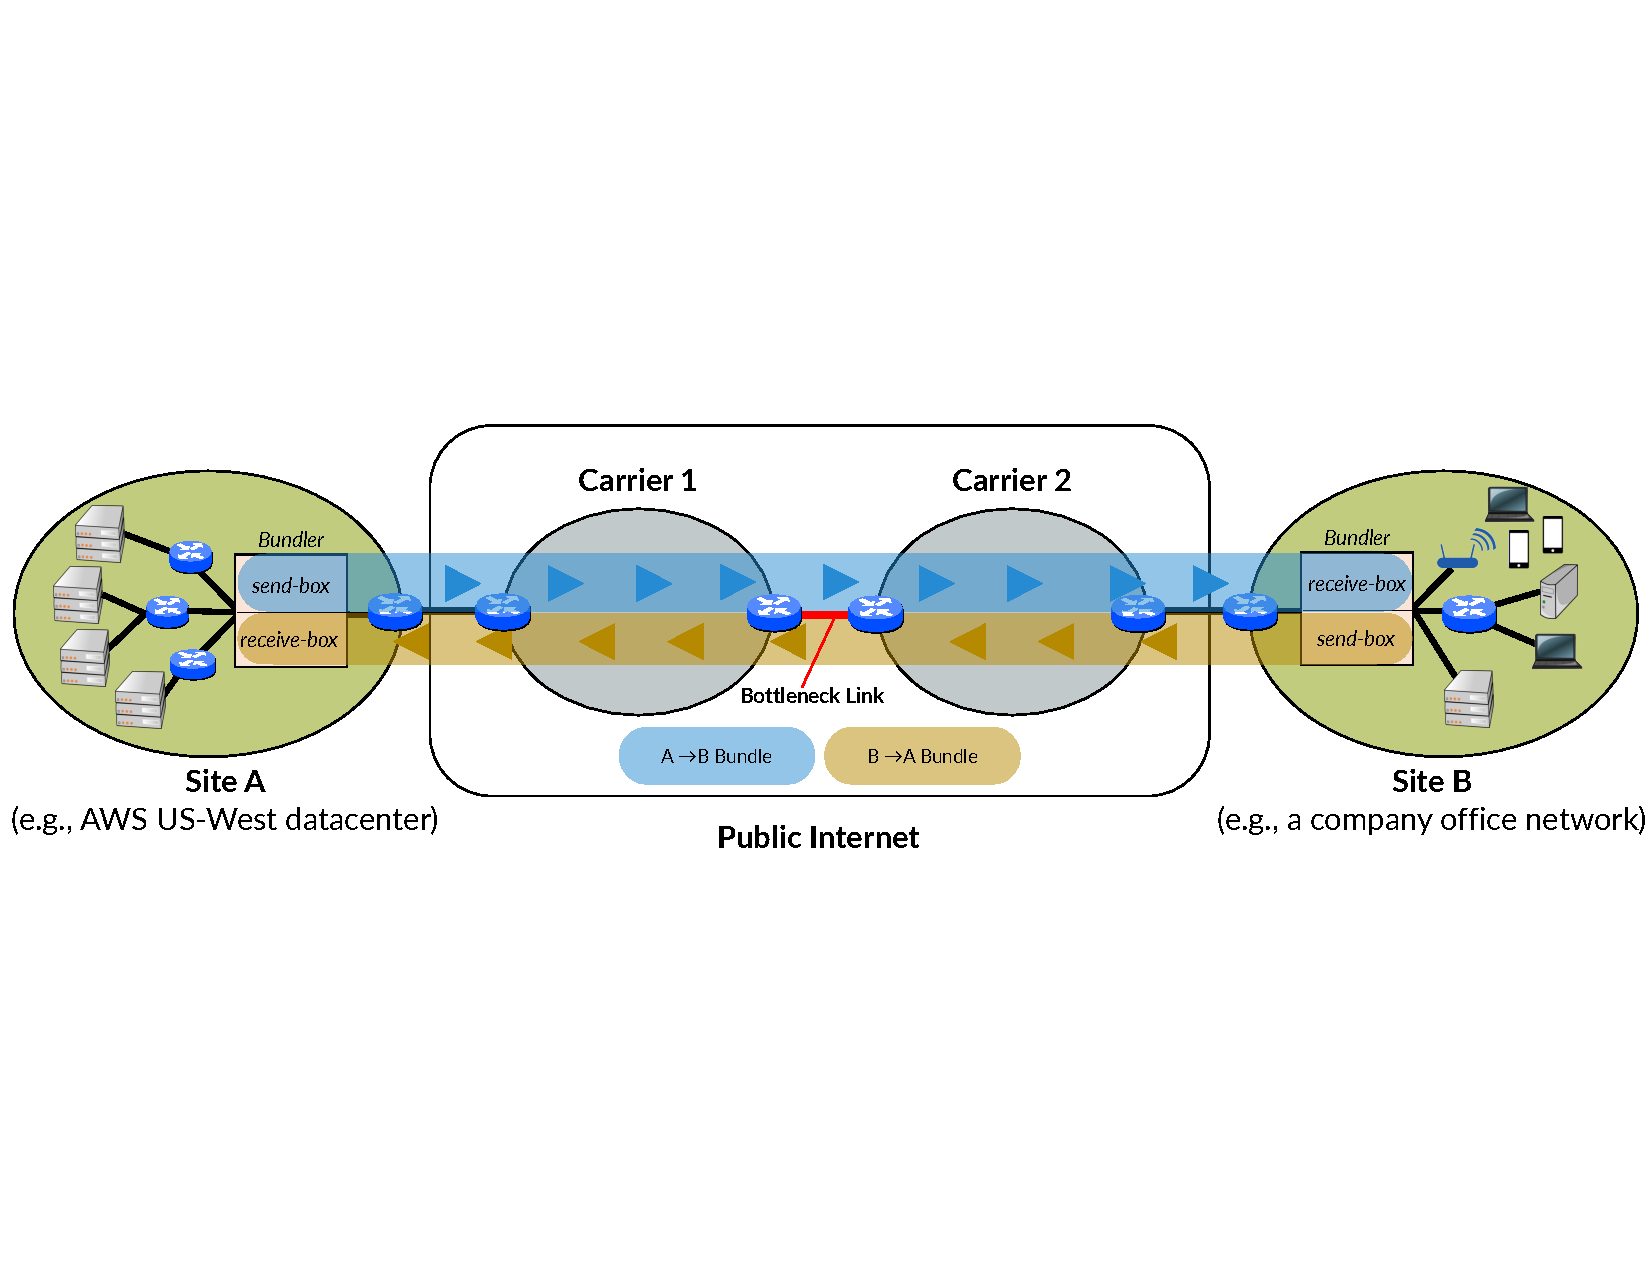
\includegraphics[width=\textwidth]{img/deployment-arch.pdf}
    \caption{An example deployment scenario for \name. 
    \name sits at each domain's edge. Traffic between the two boxes is aggregated into a single unidirectional bundle, shown as shaded boxes. The \inbox schedules the traffic within the bundle according to the policy the sending domain specifies (\S\ref{s:design}).
    }\label{fig:deploy:arch}
\end{figure*}

%We further note that middleboxes are now prevalent in the Internet architecture~\cite{aplomb}. They are often deployed at the egress and ingress of a network domain, to ensure traffic transits them for intrusion detection, packet inspection, filtering etc. They thus provide an effective vantage point for aggregating and managing traffic. 
To move the queues and schedule traffic bundles, we propose a new type of middlebox, called \name, that (1) dynamically aggregates the traffic at the content provider's egress into appropriate bundles, (2) does rate control for each bundle to move the corresponding queues from within the network to itself, and (3) applies scheduling and AQM policies within each bundle. 

Each domain must deploy one middlebox, which is logically composed of sender-side (\inbox) and receiver-side (\outbox) functionality;
a \emph{bundle} is a group of flows traversing the same \inbox{}-\outbox{} pair.
The bulk of \name's functionality resides at the \inbox, which coordinates with the \outbox to identify bundles and measure congestion signals such as the round-trip time and the rate at which packets are received.
The \inbox passes these signals to a congestion control algorithm (requiring certain properties described in \S\ref{s:design}) which computes appropriate sending rates for each bundle. 
By varying the sending rate, the \inbox ensures that the queuing induced by the bundled traffic within the network is low and is incurred at the \inbox instead, while maintaing high utilization at the bottleneck link.
 
We introduce a lightweight method for the coordination between the \inbox and the \outbox which does not require any per-flow state and can be deployed in a mode that forwards packets without modification. \name requires no changes to the end hosts or to the routers in the network.
 
Note that our goal is to perform scheduling and queue management only on the traffic within the same bundle. We do not currently attempt to control traffic across different bundles. 
Furthermore, as we will discuss in \S\ref{s:deploy}, there may be instances where \name cannot improve performance for the bundled traffic, and falls back to the status quo performance. 
Despite these limitations, we believe that our work provides a deployable solution for enabling some of the benefits of scheduling and queue management in the Internet from the edge of the content provider's network.
 
We make the following contributions:
\begin{enumerate}
    \item A ligh-weight, scalable, and deployable architecture that enables content providers to perform scheduling across traffic with a common destination domain. In this architecture, content providers perform congestion control over bundles of traffic with a common destination domain in order to move queueing to the content provider's edge (\S\ref{s:design}).
     \item A novel low-overhead protocol-agnostic technique for measuring signals for congestion control between the \pair, that need not make any changes to the packet headers (\S\ref{s:measurement}).
     \item A new congestion controller, synthesized from existing building blocks in congestion control (delay-control, AQM, and cross-traffic inference) for use with traffic bundles (\S\ref{s:queue-ctl}).
     %\item The design and implementation of a \name, including a novel method of collecting congestion control information and enforcing the decisions of a rate control algorithm on traffic aggregates, which \emph{moves} the queues from the bottleneck in the network to the customer's edge.
     %\item An evaluation of the benefits of scheduling and queue management for traffic aggregates, compared to both the status quo (FIFO) and an idealized deployment where bottleneck queues deploy the desired policy.
\end{enumerate}
